\subsection{Tipos de Algoritmos}
Os atributos presentes nos dados podem ser utilizados com a premissa de predizer uma determinada hipótese. A aprendizagem supervisionada, como pode-se observar na figura \ref{fig:supervisedlearning}, justifica-se por separar o conjunto de dados em duas bases: teste e treinamento, posteriormente, utilizar as bases para produzir um modelo de predição capaz de satisfazer uma hipótese. Usualmente dentro da aprendizagem supervisionada existe um método que consiste em utilizar de um atributo discreto ou qualitativo e a partir de um indutor gerar o melhor classificador para aquele problema, esse método é chamado classificação. Ainda existe um outro, que se baseia em atributos contínuos, com isso é possível utilizar de predição numérica afim de identificar um modelo dentro do plano cartesiano e prever futuros valores para o mesmo atributo em outras situações, esse método se chama regressão. \cite{hastie2009unsupervised, russell2003artificial}

\begin{figure}[H]
    \centering
    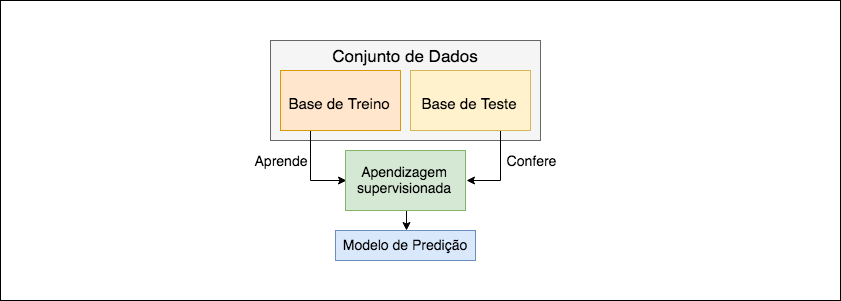
\includegraphics[width=.8\textwidth]{imagens/supervisedlearning.png}
    \caption{Diagrama representando os eventos da aprendizagem supervisionada.}
    \label{fig:supervisedlearning}
\end{figure}

Em contrapartida, existem casos onde os atributos não estarão anotados e a IA terá que literalmente inferir a probabilidade em toda a base. Esse estilo de aprendizagem se chama aprendizagem não-supervisionada, e o enfoque é utilizar da segregação dos atributos e suas dimensões para inferir resultados. O método mais comum dentro desse estilo é a clusterização que, exemplificado na figura \ref{fig:unsupervised}, se baseia em particionar os dados em grupos dentro de um plano cartesiano tomando de referencia um ou mais atributos. Outra pratica utilizada nesse tipo de aprendizagem é redução dimensional, onde resume-se o estado atual de um item para um estado de menor complexidade de dimensões com base nas propriedades chaves \cite{hastie2009unsupervised, mohri2012foundations}.

\begin{figure}[H]
    \centering
    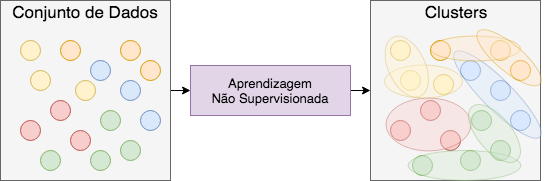
\includegraphics[width=.8\textwidth]{imagens/unsupervised.png}
    \caption{Diagrama representando a clusterização.}
    \label{fig:unsupervised}
\end{figure}

Ainda correlacionado com as últimas explicações, existe um tipo onde é inserido no agente dados anotados e não anotados para predição de todos os itens da base. A aprendizagem semi-supervisionada, sucintamente definida, é a mescla das duas outras aprendizagens. Utiliza da parte anotada (supervisionada) e da lógica de grupos (não-supervisionada), para normalizar e otimizar o resultado final \cite[7]{mohri2012foundations}.

Por último, existem casos onde não teremos dados suficientes para executar outros tipos de aprendizagem, nesse momento a aprendizagem baseada na tradicional tentativa e erro. Nomeada aprendizado por reforço, se observar a \ref{fig:reinforcement} pode-se notar que se, consiste em um ambiente (A), responsável por emitir um estado para o componente, feito isso é aplicado uma entrada de dados (e) ao nosso agente (G) que será responsável por tomar a decisão de que ação (a) tomara para a entrada (e) previamente recebida. Essa ação modifica o estado do ambiente e transmite um sinal de reforço visando através do componente (r) para que a aplicação tome a melhor escolha ao longo prazo \cite{kaelbling1996reinforcement, russell2003artificial}.

\begin{figure}[H]
    \centering
    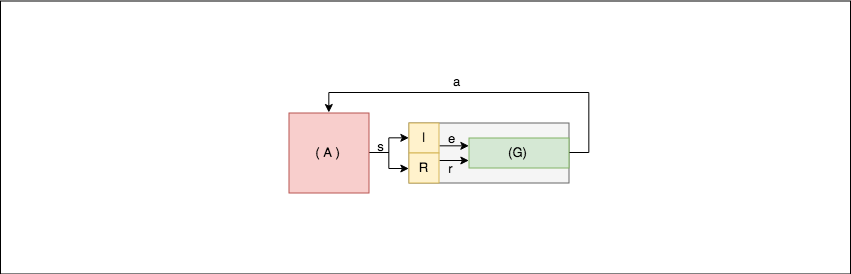
\includegraphics[width=.8\textwidth]{imagens/reinforcement.png}
    \caption{Diagrama apresentando o modelo sequencia ocorrido durante a aprendizagem por reforço.}
    \label{fig:reinforcement}
\end{figure}

Indiferente do tipo ou situação em que o algoritmo se enquadra, a multiplicidade de escolhas propostas pelo \textit{machine learning} gerou várias propostas de aprendizado, algumas até tentando utilizar da estrutura proposta pela neurociência para replicar nossas redes neurais.
